\hsection{Fixed:~Transitive Dependency factored out into own Table}%
\FloatBarrier%
%
\begin{figure}%
\centering%
%
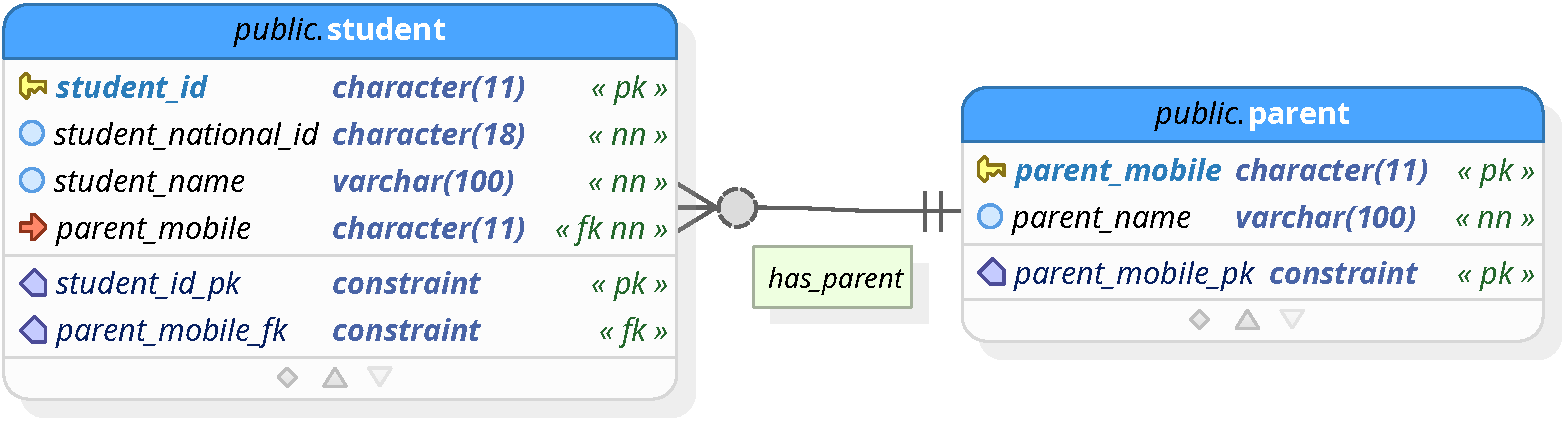
\includegraphics[width=0.56\linewidth]{\currentDir/studentFixed3nf}%
%
\caption{Two tables which store data about students and their parents and which, different from \cref{fig:studentViolation3nf}, do not violate the \pgls{3NF}.}%
\label{fig:studentFixed3nf}%
\end{figure}%
%
\gitExec{\databasesCodeRepo}{.}{_scripts_/postgres.sh normalization/3nf/student/fixed/generated_sql 01_fixed_database_2001.sql}%
%
\gitSQL{\databasesCodeRepo}{normalization/3nf/student/fixed/generated_sql/03_public_student_table_5071.sql}{3nf:student:fixed:03_public_student_table_5071}{The generated \sql\ code for creating the table \sqlil{student}.}%
\gitExec{\databasesCodeRepo}{.}{_scripts_/postgres.sh normalization/3nf/student/fixed/generated_sql 03_public_student_table_5071.sql fixed}%
%
\gitSQL{\databasesCodeRepo}{normalization/3nf/student/fixed/generated_sql/04_public_parent_table_5079.sql}{3nf:student:fixed:04_public_parent_table_5079}{The generated \sql\ code for creating the table \sqlil{parent}.}%
\gitExec{\databasesCodeRepo}{.}{_scripts_/postgres.sh normalization/3nf/student/fixed/generated_sql 04_public_parent_table_5079.sql fixed}%
%
\gitSQL{\databasesCodeRepo}{normalization/3nf/student/fixed/generated_sql/05_public_student_parent_mobile_fk_constraint_5090.sql}{3nf:student:fixed:05_public_student_parent_mobile_fk_constraint_5090}{We add the foreign key constraint to table~\sqlil{student}.}%
\gitExec{\databasesCodeRepo}{.}{_scripts_/postgres.sh normalization/3nf/student/fixed/generated_sql 05_public_student_parent_mobile_fk_constraint_5090.sql fixed}%
%
\gitSQL{\databasesCodeRepo}{normalization/3nf/student/fixed/insert.sql}{3nf:student:fixed:insert}{%
Inserting some data into the tables~\sqlil{parent} and~\sqlil{student}.}%
\gitExec{\databasesCodeRepo}{.}{_scripts_/postgres.sh normalization/3nf/student/fixed insert.sql fixed}%
%
\gitSQLAndOutput{\databasesCodeRepo}{normalization/3nf/student/fixed}{select.sql}{fixed}{}{}{postgres.sh}{3nf:student:fixed:select}{%
If we want to get the names of the parents of the students, we now need an~\sqlilIdx{INNER JOIN}.%
}%
%
\gitSQLAndOutput{\databasesCodeRepo}{normalization/3nf/student/fixed}{update.sql}{fixed}{}{}{postgres.sh}{3nf:student:fixed:update}{%
We noticed that the name of the father of Mr.~Bibbo, Mr.~Bibotto, and Ms.~Bibboba is actually Mr.~B{\"o}dd{\"o}, not Mr.~Boddo. %
Since we now observe the \pgls{3NF}, we need to touch only a single records to change this.%
}%
%
%
In \cref{fig:studentFixed3nf} we illustrate a logical model that no longer violates the \pgls{3NF}.
Different from our original sketch in \cref{fig:studentViolation3nf}, we use two tables instead of one.
The name of the parent depends on their mobile phone number.
So we remove this data from the original \sqlil{student}~table and put it into a table~\sqlil{parent}.
This table has the primary key~\sqlil{parent_mobile}.
This value is unique and identifies a parent.
The second column of this table~\sqlil{name}, which obviously depends on that primary key.

The modified table~\sqlil{student} now uses the attribute~\sqlil{parent_mobile} as foreign key.
It must be \sqlilIdx{NOT NULL}, meaning that each row in table~\sqlil{student} is linked to one~(and exactly one) row in table~\sqlil{parent}.
We now no longer store the name of the parent in the \sqlil{student}~table.

Both tables observe the \pgls{1NF}, as there are neither compound attributes nor repeated groups.
Both also observe the \pgls{2NF}, because there is no compound key and, hence, it is not possible that an attribute could depend on a part of such a key only.
They also both observe the \pgls{3NF}, because there is no transitive functional dependency.

Let us look at this system in action.
We first create the table~\sqlil{student} by executing the script given in \cref{lst:3nf:student:fixed:03_public_student_table_5071}.
\Cref{lst:3nf:student:fixed:04_public_parent_table_5079} then creates the new table~\sqlil{parent} for the parent records.
With \cref{lst:3nf:student:fixed:05_public_student_parent_mobile_fk_constraint_5090}, we add the foreign key constraint to table~\sqlil{student}.
Like the \db\ creation and deletion scripts, sometimes I will just not include such constraint-creation steps, as they are not very relevant to the example.
They can always found in the corresponding example directory in the repository \href{\xdef\databasesCodeRepo}{\databasesCodeRepoName} with the complete examples.
This time I felt like including it, just for the sake of completeness.

Anyway, we can now insert data into this new \db\ structure.
In \cref{lst:3nf:student:violation:insert}, we begin by storing the two parent records into the table~\sqlil{parent}.
The mobile phone numbers and names of Ms.~Balla, the mom of Mr.~Bebbo, as well as Mr.~B{\"o}dd{\"o}, the dad of the other three students are stored.
Then we insert four student records for Mr.~Bibbo, Mr.~Bebbo, Mr.~Bibboto, and Ms.~Bibboba.
Like last time, our data entry specialist did, at first, not know how to write the the fancy~\inQuotes{\"o} in name Mr.~B{\"o}dd{\"o} and resorted to just call him~Mr.~Boddo.

At first glance, this new structure looks more complicated.
On one hand, we now have two tables instead of one.
On the other hand, if we want to know the names of the parents of the students, a simple~\sqlilIdx{SELECT} will no longer be enough.
Instead, we need to merge the data from two tables by using an~\sqlilIdx{INNER JOIN}, as shown in \cref{lst:3nf:student:fixed:select}.

One could argue that the advantage is the reduced redundancy:
The name of each parent is entered once and only one.
Then again, you may argue that in this simple example, this advantage is more or less offset by the fact that we need to enter their mobile phone numbers in both tables.
Generally, the redundancy reduction is still a good argument.

The usefulness of the new design becomes clear when we change data.
Like in our original example, a few days after originally entering the data, our data entry specialist found a solution on how to enter the letter~\inQuotes{\"o}.
In order to fix the data, they created the script \cref{lst:3nf:student:violation:update}.
The \sqlilIdx{UPDATE} command is now applied to table~\sqlil{parent} and only touches a single row~(as you can see by the result of the \sqlilIdx{RETURNING} statement).
In the same script, we use another \sqlilIdx{SELECT} to check whether the parent names of Mr.~Bibbo, Mr.~Bibboto, and Ms.~Bibboba have changed.
And indeed, they have.
The update anomaly has disappeared.

The new design also no longer would exhibit a deletion anomaly, as we can delete student records without losing the information about the parents.
We can also insert new parent records at any time, without requiring that student records of their kids are already present, so there is no insertion anomaly either.%
%
\FloatBarrier%
\endhsection%
%
